\documentclass[xcolor=table]{article}
\usepackage{DejaVuSansMono}
\usepackage{ragged2e}
\usepackage{csquotes}
\usepackage{pstricks}
\usepackage{pst-text}
\usepackage{pst-node}
\usepackage{pst-eps}
\usepackage{savesym}
\savesymbol{checkmark}
\usepackage{dingbat}
\usepackage{anyfontsize}
\usepackage{pifont}
\usepackage{wasysym}
\usepackage{graphicx}
\begin{document}
\psset{unit=1.5in}
\fontfamily{DejaVuSansMono-TLF}\fontsize{80}{80}\selectfont%
\TeXtoEPS
\begin{pspicture}(0,0)(3,6)
%\rput[bl](0,0){\psgrid(0,0)(3,6)}
\rput[bl](0.5,0.5){\includegraphics{pn2222.eps}}
\rput[bl](0.80,0.45){E}
	\rput[bl](1.4,0.15){\textcolor{blue}{C}}
	\rput[bl](2.1,0.10){\textcolor{red}{B}}
\end{pspicture}
\endTeXtoEPS
\end{document}
